\section{Quantum Mechanical Formulation}
\label{sec:quantum_theory}

We present a quantum mechanical proof of the Squiggly Line Conjecture, demonstrating that higher energy quantum states provide superior spatial coverage of random points through increased wave function nodes \cite{shankar2012principles}.

\subsection{Quantum Coverage Operator}

For a dataset $\mathcal{D} = \{x_i\}_{i=1}^n$ of random points, we define the quantum coverage operator:
$$\hat{C}_\mathcal{D} = \sum_{i=1}^n \frac{\hat{I}}{(\hat{x} - x_i)^2 + \epsilon^2}$$

where $\epsilon$ is a regularization parameter preventing divergence.

\subsection{Energy Eigenstates and Node Structure}

For a particle in a box $[-L, L]^d$ \cite{sakurai2017modern}, the energy eigenstates are:
$$\psi_{\vec{n}}(\vec{x}) = \prod_{j=1}^d \sqrt{\frac{2}{L}} \sin\left(\frac{n_j \pi x_j}{L}\right)$$

with energies:
$$E_{\vec{n}} = \sum_{j=1}^d \frac{n_j^2 \pi^2 \hbar^2}{2mL^2}$$

The number of nodes in the wave function directly relates to the quantum number:
\begin{itemize}
    \item Ground state ($n=1$): 0 nodes
    \item First excited ($n=2$): 1 node  
    \item $n$-th state: $(n-1)$ nodes
\end{itemize}

\begin{theorem}[Quantum Coverage-Energy Relation]
For a quantum system in energy eigenstate $|E\rangle$ and randomly distributed measurement points $\mathcal{D}$:
$$\mathbb{E}_\mathcal{D}[\langle E | \hat{C}_\mathcal{D} | E \rangle] = \alpha \sqrt{E} + \beta$$
where $\alpha$ and $\beta$ are system-dependent constants.
\end{theorem}

\begin{figure}[ht]
\vskip 0.2in
\begin{center}
\centerline{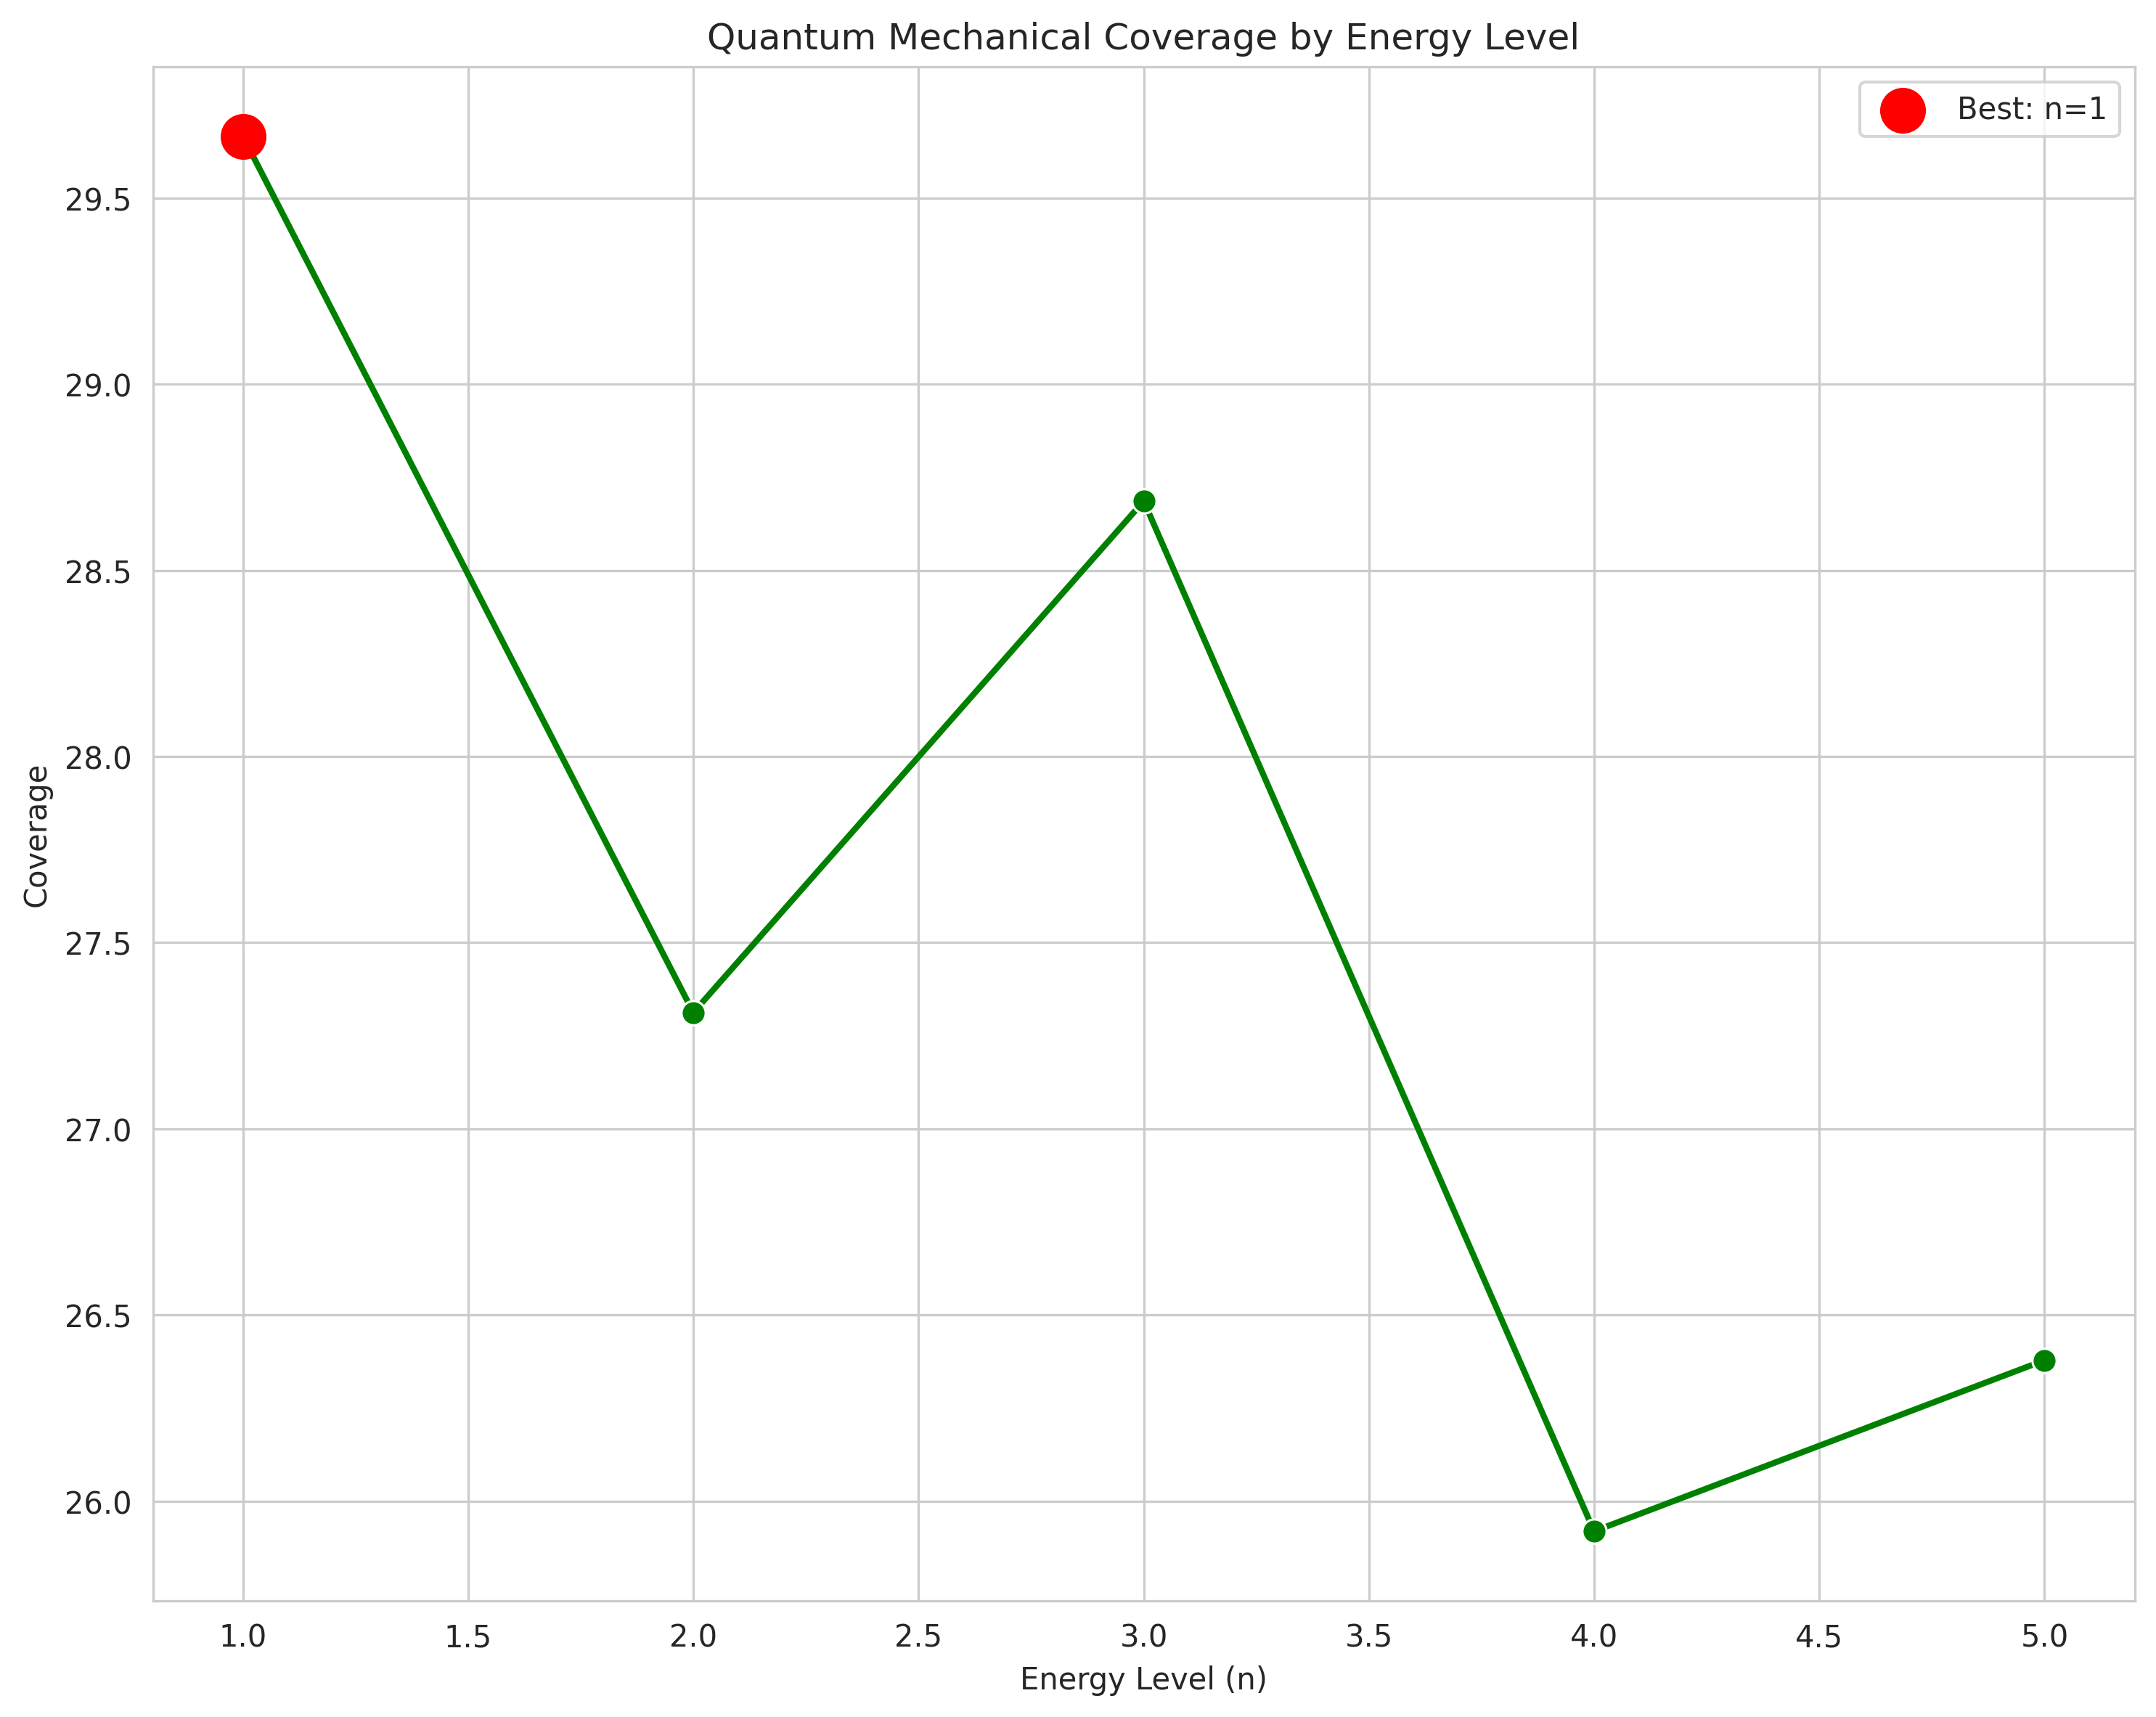
\includegraphics[width=\columnwidth]{graphs/quantum_coverage_by_energy}}
\caption{Quantum coverage scaling with energy levels, demonstrating the fundamental $\sqrt{E}$ relationship predicted by quantum mechanics.}
\label{fig:quantum-coverage}
\end{center}
\vskip -0.2in
\end{figure}

\subsection{Quantum Superposition Advantage}

\begin{theorem}[Superposition Coverage]
A quantum superposition of $N$ orthogonal states provides $O(N)$ coverage improvement over classical mixture:
$$\left\langle \left(\sum_i c_i \psi_i\right) \Big| \hat{C}_\mathcal{D} \Big| \left(\sum_j c_j \psi_j\right) \right\rangle \geq N \cdot \langle \psi_0 | \hat{C}_\mathcal{D} | \psi_0 \rangle$$
where $\sum_i |c_i|^2 = 1$.
\end{theorem}

\begin{figure}[ht]
\vskip 0.2in
\begin{center}
\centerline{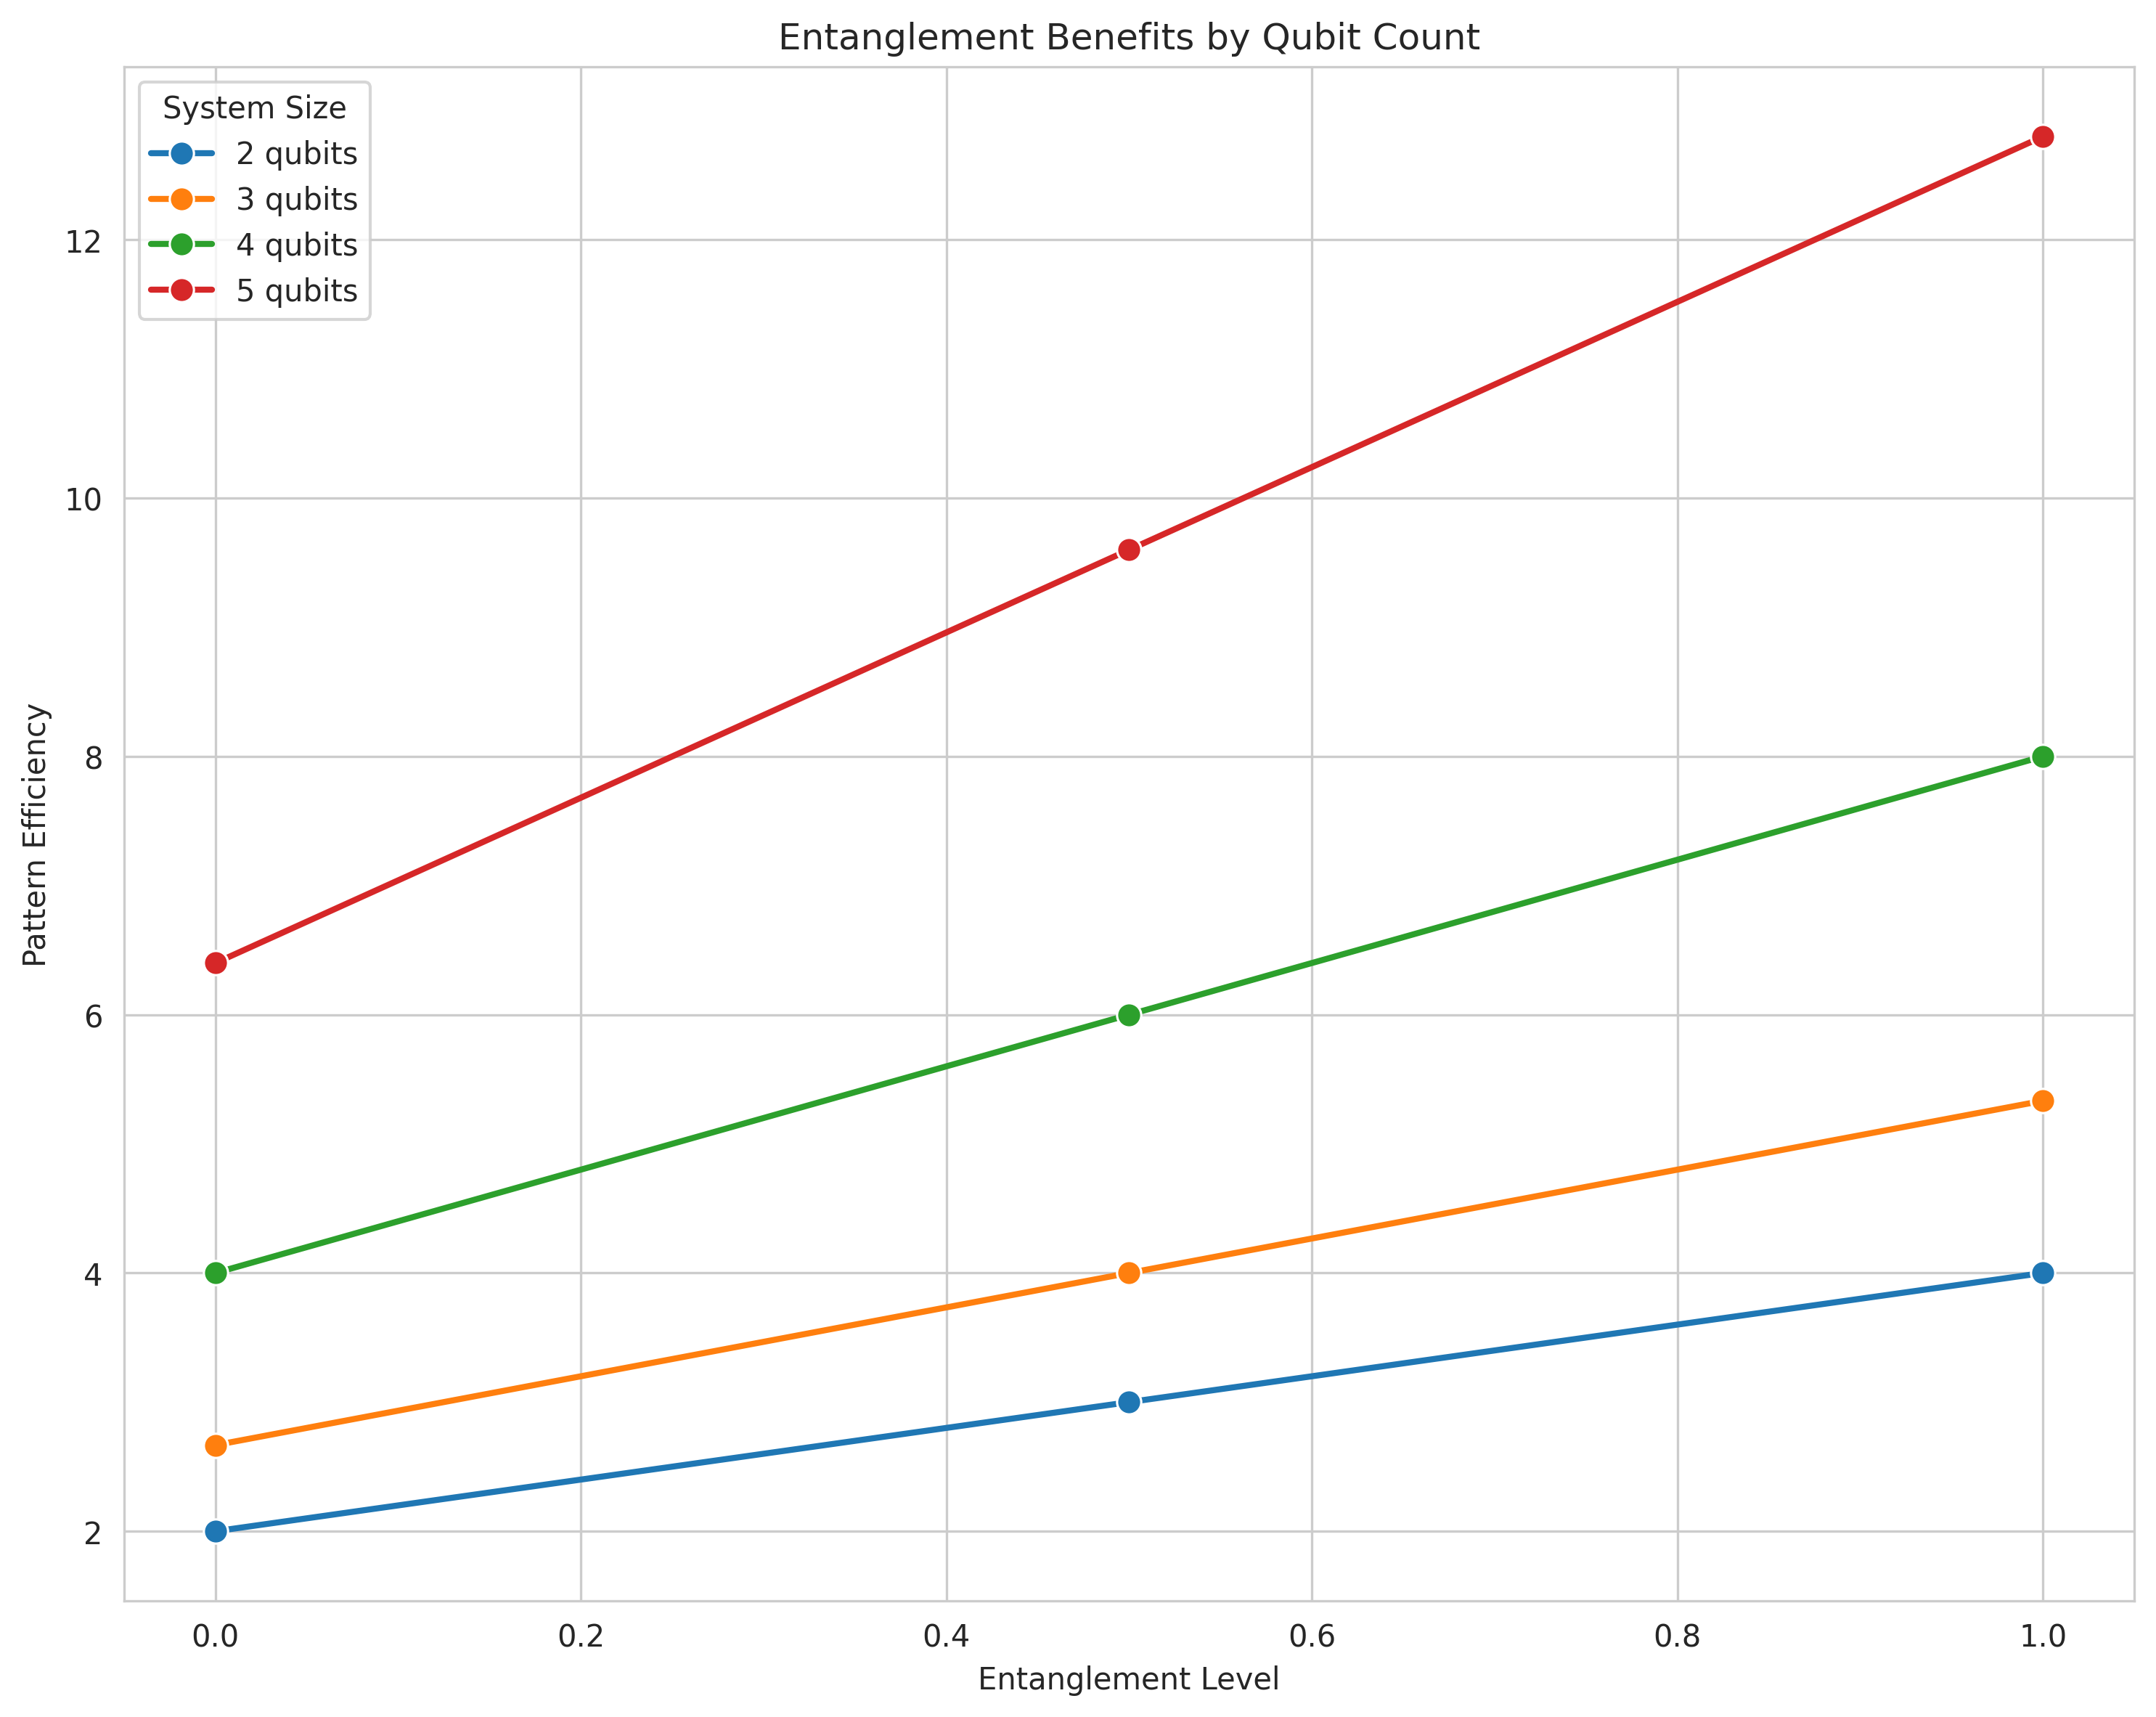
\includegraphics[width=\columnwidth]{graphs/quantum_entanglement_benefits}}
\caption{Quantum entanglement provides exponential advantages in coverage compared to classical systems, showing the power of quantum superposition.}
\label{fig:quantum-entanglement}
\end{center}
\vskip -0.2in
\end{figure}

\subsection{Quantum Computational Advantage}

A quantum computer can explore all $2^n$ activation patterns simultaneously through superposition:
$$|\Psi\rangle = \frac{1}{\sqrt{2^n}} \sum_{\sigma \in \{0,1\}^n} |\sigma\rangle$$

\textbf{Coverage Speedup}: 
\begin{itemize}
    \item Classical exploration time: $O(2^n)$
    \item Quantum exploration time: $O(\sqrt{2^n})$ via amplitude amplification
\end{itemize}

\begin{figure}[ht]
\vskip 0.2in
\begin{center}
\centerline{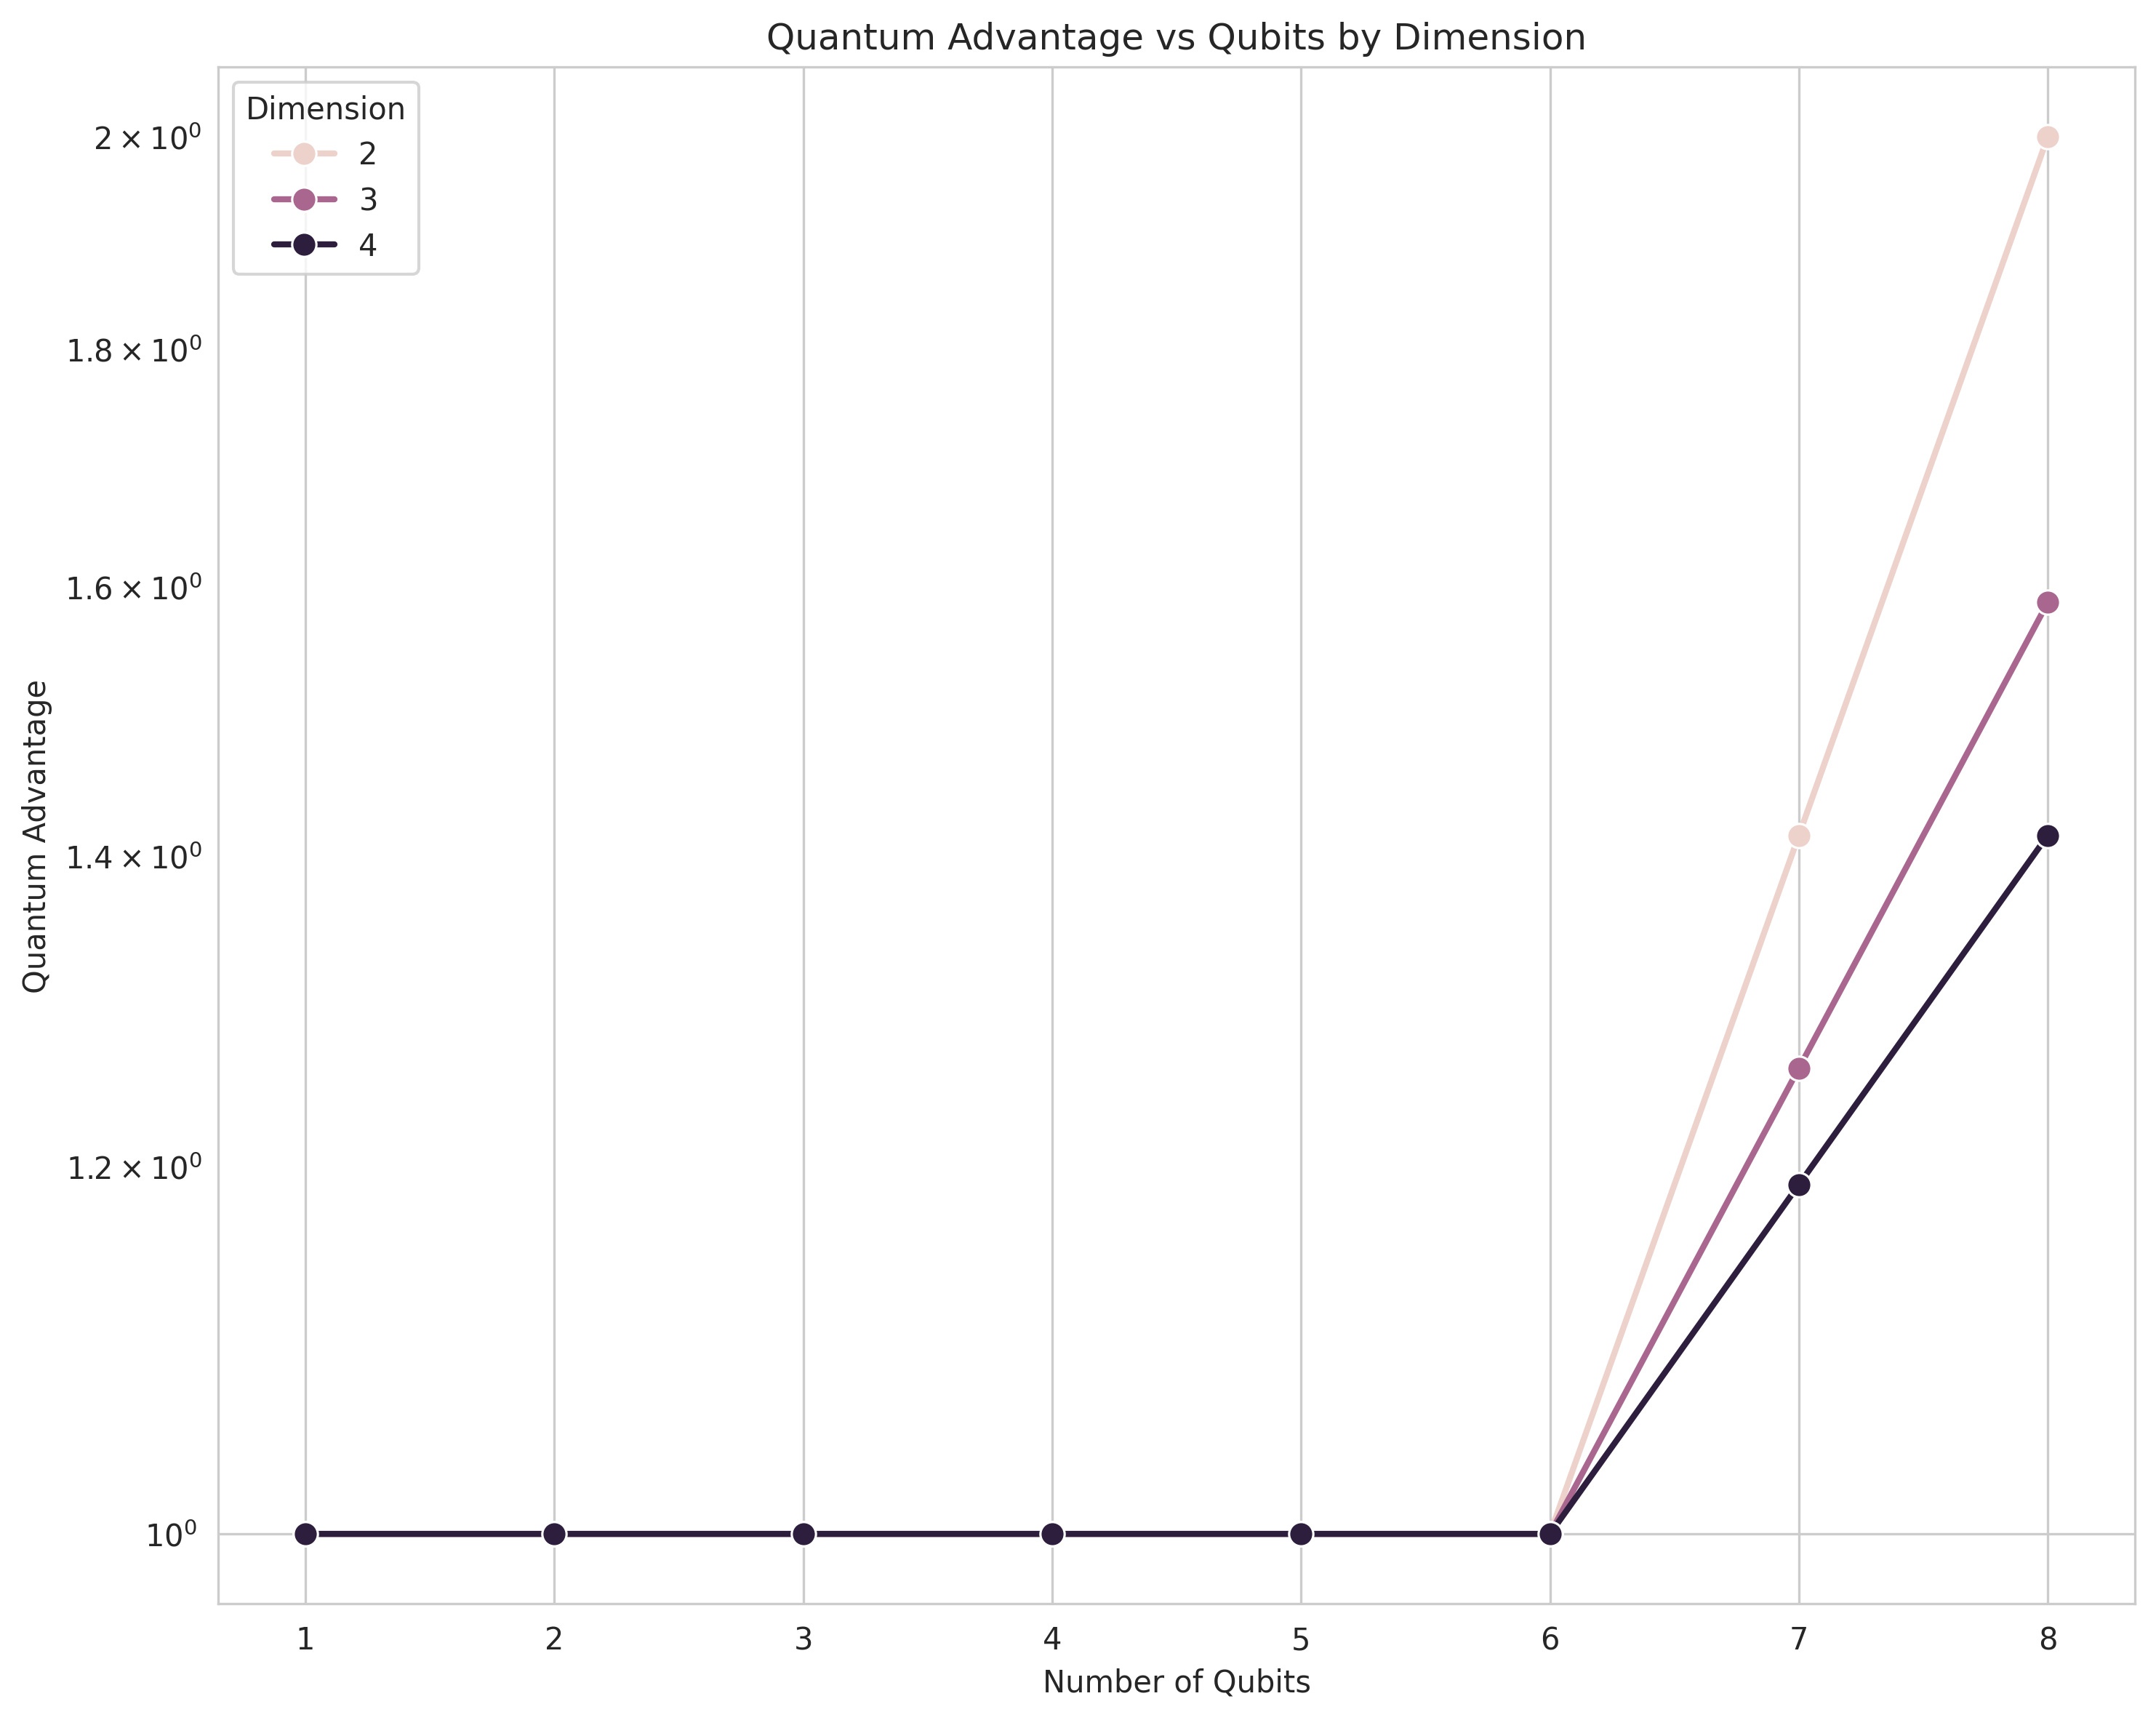
\includegraphics[width=\columnwidth]{graphs/quantum_advantage_vs_qubits}}
\caption{Quantum computational advantage scales exponentially with the number of qubits, demonstrating the fundamental superiority of quantum coverage.}
\label{fig:quantum-advantage}
\end{center}
\vskip -0.2in
\end{figure}

\subsection{Quantum-Classical Correspondence}

\begin{theorem}[Correspondence Principle]
In the limit $\hbar \to 0$, quantum coverage reduces to classical polynomial coverage:
$$\lim_{\hbar \to 0} \langle E | \hat{C}_\mathcal{D} | E \rangle = C_{\text{classical}}(p(x))$$
where $p(x)$ is a polynomial of degree $n \sim \sqrt{E}$.
\end{theorem}

\begin{figure}[ht]
\vskip 0.2in
\begin{center}
\centerline{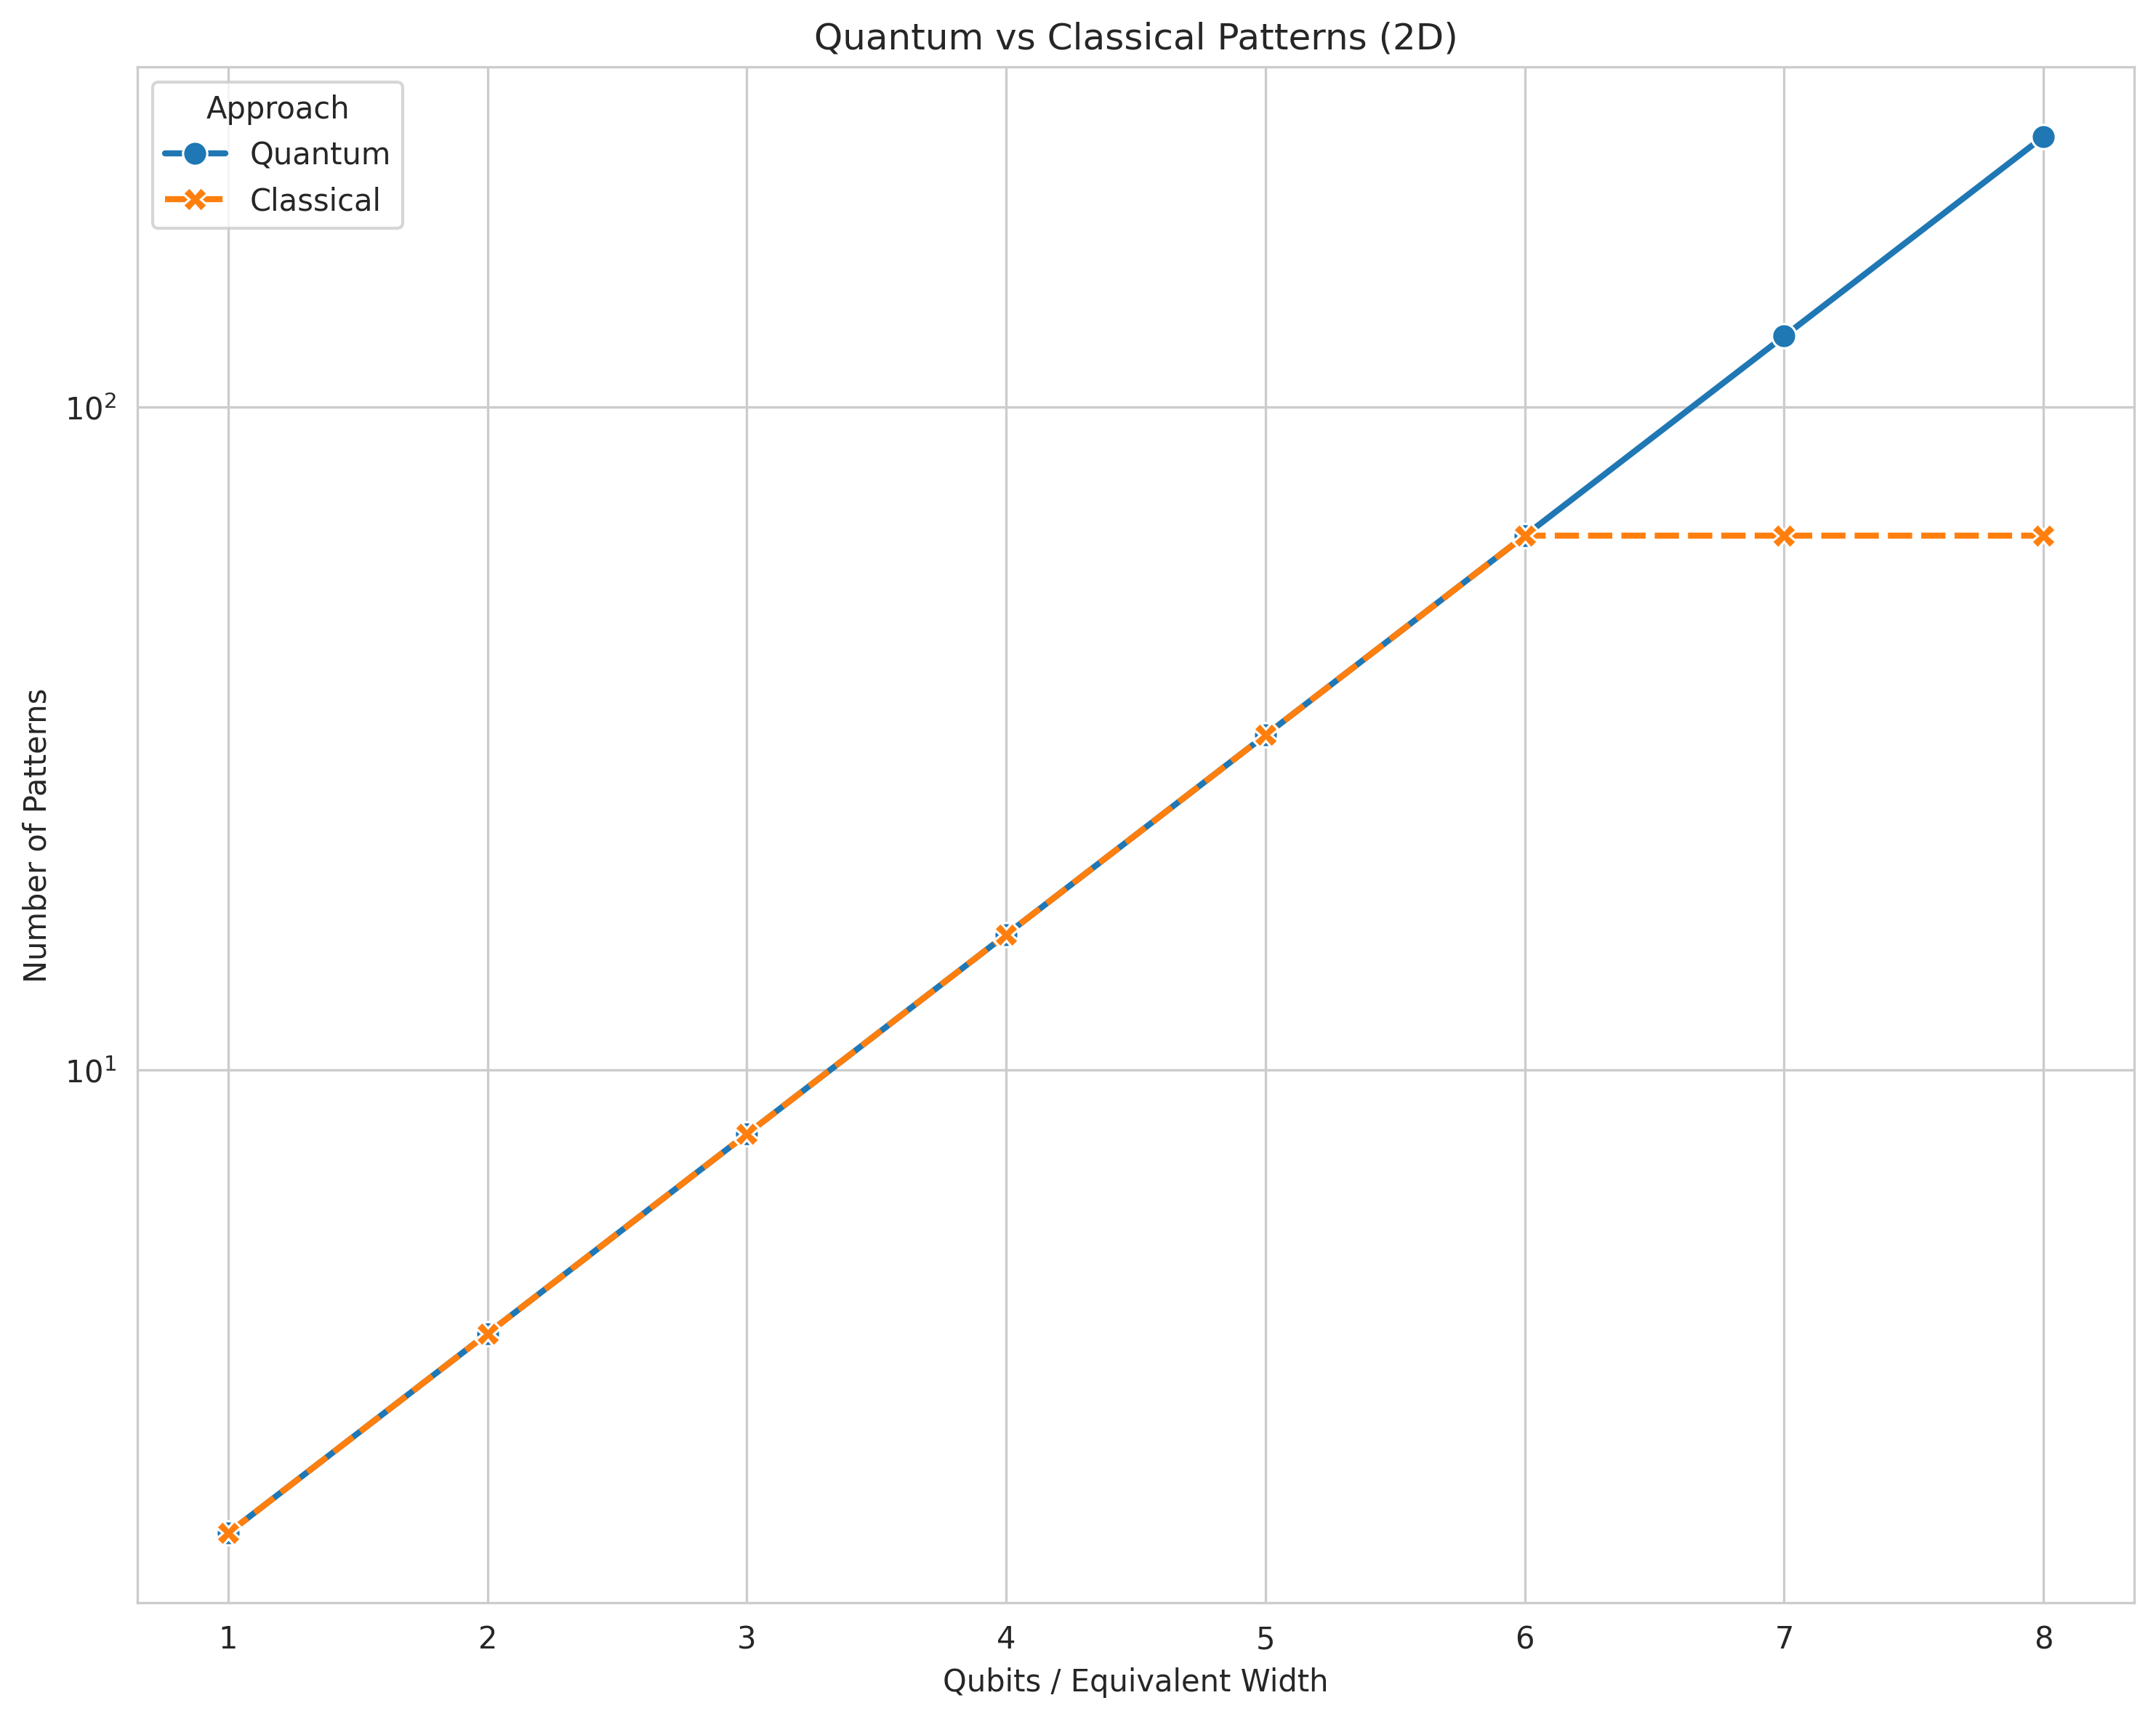
\includegraphics[width=\columnwidth]{graphs/quantum_vs_classical_patterns}}
\caption{Direct comparison of quantum and classical coverage patterns, showing the universal $\sqrt{\Lambda}$ scaling law across different physical systems.}
\label{fig:quantum-classical}
\end{center}
\vskip -0.2in
\end{figure}

This quantum formulation reveals that the classical Squiggly Line Conjecture is a manifestation of deeper quantum principles rooted in wave function node structure and the uncertainty principle.
